% !TEX TS-program = pdflatex
% !TEX encoding = UTF-8 Unicode

% This is a simple template for a LaTeX document using the "article" class.
% See "book", "report", "letter" for other types of document.

\documentclass[11pt]{article} % use larger type; default would be 10pt

\usepackage[utf8]{inputenc} % set input encoding (not needed with XeLaTeX)

%%% Examples of Article customizations
% These packages are optional, depending whether you want the features they provide.
% See the LaTeX Companion or other references for full information.

%%% PAGE DIMENSIONS
\usepackage{geometry} % to change the page dimensions
\geometry{a4paper} % or letterpaper (US) or a5paper or....
\geometry{margin=1in} % for example, change the margins to 2 inches all round
% \geometry{landscape} % set up the page for landscape
%   read geometry.pdf for detailed page layout information

\usepackage{graphicx} % support the \includegraphics command and options

% \usepackage[parfill]{parskip} % Activate to begin paragraphs with an empty line rather than an indent

%%% PACKAGES
\usepackage{booktabs} % for much better looking tables
\usepackage{array} % for better arrays (eg matrices) in maths
\usepackage{paralist} % very flexible & customisable lists (eg. enumerate/itemize, etc.)
\usepackage{verbatim} % adds environment for commenting out blocks of text & for better verbatim
\usepackage{subcaption} % make it possible to include more than one captioned figure/table in a single float
% These packages are all incorporated in the memoir class to one degree or another...

\usepackage[lighttt]{lmodern}
\ttfamily
\DeclareFontShape{OT1}{lmtt}{m}{it}
     {<->sub*lmtt/m/sl}{}
\usepackage{xcolor}
\usepackage{mathtools}
\usepackage{amsmath}

%\usepackage[font=small,labelfont=bf]{subcaption}

%%% HEADERS & FOOTERS
\usepackage{fancyhdr} % This should be set AFTER setting up the page geometry
\pagestyle{fancy} % options: empty , plain , fancy
\renewcommand{\headrulewidth}{0pt} % customise the layout...
\lhead{}\chead{}\rhead{}
\lfoot{}\cfoot{\thepage}\rfoot{}

\captionsetup{font+=small}

%%% END Article customizations

%%% The "real" document content comes below...
\begin{document}

\section{Model}

These simulations of the intestinal crypt are performed using cell based models in CHASTE \cite{Mirams2013}, discussed in \cite{VanLeeuwen2009}. A cylindrical approximation to the crypt is modelled using a 2D rectangle with periodic boundary condtions on the left and right and sides. A gradient of Wnt signalling factor (highest at the bottom of the crypt) is imposed on a   subcellular Wnt signalling model, which provides input to  the cell cycle model \cite{Swat2004}. This model is then coupled to the Meineke \textit{et al} model \cite{Meineke2001}, see Figure \ref{fig:Multiscale_Model}, which deals with the multicellular interactions, including cell division, differentiation and cell migration.

\begin{figure}
\centering
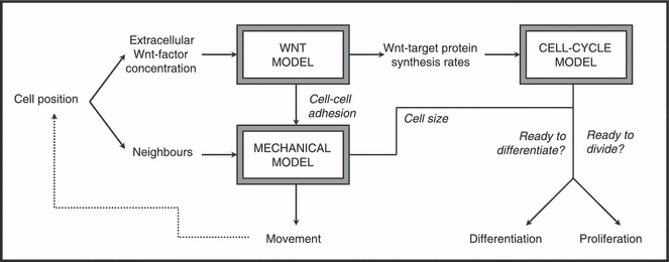
\includegraphics[width=0.8\textwidth]{Model_Summary}
\caption{Schematic of the multiscale model for the dynamics of a colonic crypt. During a model simulation, the occurrence of cellular events
(proliferation, differentiation, migration) is monitored at discrete time steps, $t_n$. By coupling Wnt signalling, cell cycle, and mechanical models, the spatio-temporal behaviour  of every cell is predicted at time $t_{n+1}$, given the state of the system at time $t_n$ (e.g. intracellular protein levels,
cell position, Wnt stimulus, location of neighbouring cells) and the system parameters. Figure from \cite{VanLeeuwen2009}}
\label{fig:Multiscale_Model}
\end{figure}

\subsection{Meineke \textit{et al} Model}

The model is populated with stem, transit and differentiated cells, which can undergo cellular proceses at discrete times $t_n$:
\begin{description}
\item[Cell Division]{Stem and transit cells undergo division, with a new cell cycle time being assigned to each daughter cell. The direction of division is stochastic, with one daughter cell placed at the site of the mother cell, the other a fixed distance away.}
\item[Cell Differentiation]{Stem cells divide such that one daughter cell remains a stem cell, the other becoming a transit cell. After a fixed number of generations transit cells undergo terminal differenation}
\item[Cell Death]{Cells above the top layer of the crypt are considered to have undergone cell death}
\item[Cell Migration]{Stem cells are non mobile, whereas transit and differianted cells move due to forces exerted due to cell division. The movement is modelled by overdamped springs, see figure \ref{fig:Mechanical_model}. Cell shape is determined by the cell centre ans Voronoi Tessellation.}
\end{description}

\begin{figure}
\centering
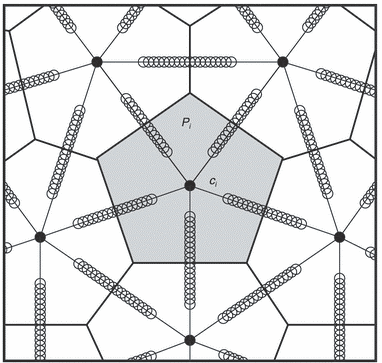
\includegraphics[width=0.4\textwidth]{Mechanical_Model}
\caption{Black points
correspond to cell centres. Each pair of neighbouring cells (identified
using a Delaunay triangulation) is attached by a spring. Solid lines
represent the associated Voronoi tessellation, which is a partition of
two-dimensional space that assigns a polygon $P_i$ to each cell centre $c_i$
such that all points in $P_i$ are closer to $c_i$ than to any other cell centre. Five
neighbouring cells surround the central cell i, highlighted in grey. Figure from \cite{VanLeeuwen2009} }
\label{fig:Mechanical_model}
\end{figure}

\subsection{Wnt Signalling}

The Wnt concentration gradient is set to be a linear function with a higher concentration at the bottom of the crypt. Each cell detects the Wnt concentration at the cell centre, the Wnt pathway is modelled by a system of nonlinaer ODEs \cite{vanLeeuwen2007}. The Wnt model returns the intracellular gene expression level for target proteins and the cellular adhesion potential.

\subsection{Cell Cycle model}

The cell cycle model is dependent on Wnt concentration, and thus cell cycle duration is positionally dependent. The cell cycle can be halted at $G_1$/S checkpoint, when Wnt levels are too low. These are considered differentiated cells, which can only become active if by local cell rearrangement they pass to a higher Wnt concentration region lower in the crypt.

\bibliography{comp_bio}{}
\bibliographystyle{plain}

\end{document}
